\documentclass[12pt,twoside,a4paper]{article}
\usepackage{diagbox}
\usepackage{graphicx}
\usepackage{subfigure}
\usepackage{url}
\usepackage{cite}  
\begin{document}
\bibliographystyle{unsrt}
\title{Using Binocular Stereo Cameras for Object Positioning}
\author{Xin Zhang}
\date{\today}
\maketitle
\section{Introduction}
 With binocular stereo cameras, we can take stereoscopic pictures, which allow us to calculate the position of the target object. In recent years, this technology has been widely applied to autonomous navigation, engineering surveying and other areas\cite{liu2009distance}. Actually, the position is obtained by \textbf{calculating the distance} from the camera(s) to the chosen object within the picture\cite{CVlife}\cite{li2016vehicle}. Therefore, we will focus on how to measure distance in the rest of this report.

\section{Distance Measurement Based on Binocular Stereo Vision}
Generally, distance measurement is performed according to the steps of \textbf{��Camera Calibration$\rightarrow$Image Matching$\rightarrow$ Geometric Calculation��}. That is, use two cameras on the same scene from different locations to obtain stereo images, through a variety of matching algorithms to find out the corresponding point in order to calculate the parallax, and then the distance from the scene can be calculated by triangulation methods and parallax theory.\\
\indent The process of geometric calculation is as follows\cite{mattoccia2011stereo}: in the ideal model, two cameras have the same specification, the same focal length, the same aperture and the same sensor area. In addition, the two cameras remain in the same plane, as shown in Fig. 1a. Then, we \textbf{convert 3D model to 2D picture} for better illustration, as shown in Fig. 1b, where $z$ stands for the distance we want to know, $f$ is the focal length and $B$ is the baseline. $P(X,Y,Z)$ stands for the target point and it's coordinates in the picture of the left and right camera are $p_l(u_l,v_l)$ and $p_r(u_r,v_r)$ respectively. We write the parallax of point $P$ as $d=u_l-u_r$. According to \textbf{the parallax theory and triangulation methods}, we can easily get that:
$$Z = z = \frac{B\times f}{d}$$
$$X = Z\times \frac{u_l}{f}$$
$$Y = Z\times \frac{v_l}{f}$$
\begin{figure}[htbp]
\centering
\subfigure[3D]{
    \includegraphics[width=2.5in]{Ideal.png}
}
\subfigure[2D]{
    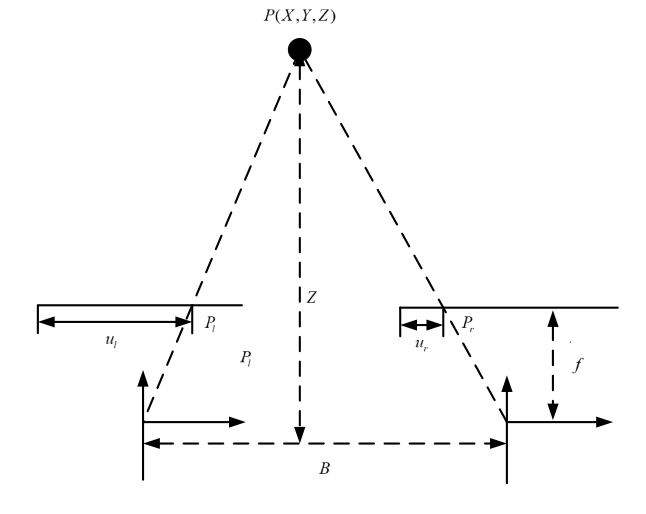
\includegraphics[width=2.5in]{ideal2D.png}
}
\caption{Ideal model}
\end{figure}
Therefore, the remaining questions are how to ensure that the two cameras meet the requirements of ideal model and how to match the imaging $p_l$ and $p_r$ of $P$ on the left and right cameras.
\subsection{Camera Calibration}
Camera calibration are critical for non-ideal model, in which two camera lenses are distorted, and the imaging planes of the left and right cameras cannot be exactly on the same plane, as shown in Fig. 2. To guarantee the accuracy of matching algorithm, we must do calibration to correct this case to ideal model as much as possible. We can use tools in OpenCV\footnote{\url{https://docs.opencv.org/3.1.0/dc/dbb/tutorial_py_calibration.html}} to calibrate directly or manually calibrate.\\
\indent In the case of using binocular stereo camera, this step can be \textbf{skipped} unless the experimental results are terrible, which means the device is too rough.
\begin{figure}
  \centering
  % Requires \usepackage{graphicx}
  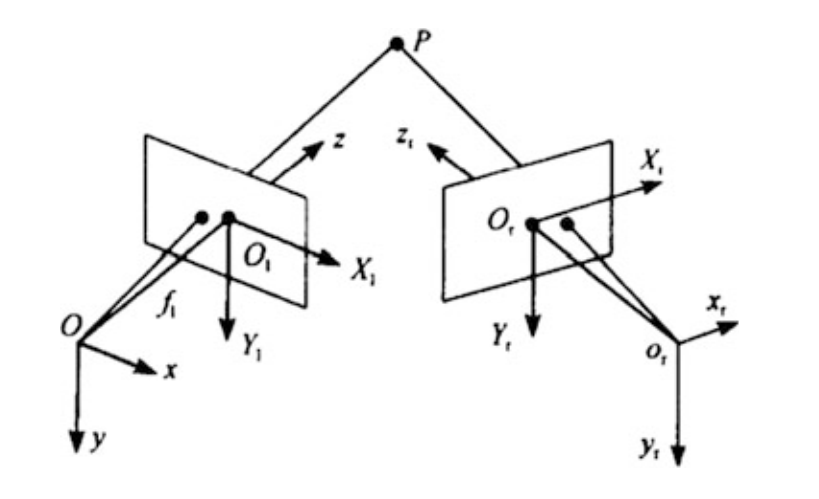
\includegraphics[width=0.6\textwidth]{nonIdeal.png}\\
  \caption{Non-ideal model}
\end{figure}

\subsection{Image Matching Problem}
Image matching is the most important step in distance measurement and we take \textbf{stereo vision algorithms} to solve this problem. These stereo vision algorithm can be divided into two categories\cite{lazaros2008review}: local methods (area-based, such as BM, SAD and so on) and global methods (energy-based, such as SGBM\footnote{strictly speaking, SGBM is semi-global method that uses both local and global approach}, GC and so on). The former is faster, while the latter is more accurate.\\
\indent In \cite{vermacomparative}, the performances of BM, GC and SGBM have been evaluated in terms of speed and quality of disparity map, the results are shown in Fig. 3 and Fig. 4. We can easily say that in terms of accuracy, GC is the best and BM is the worst, while in terms of efficiency, the opposite is true.
\begin{figure}[htbp]
\centering
\subfigure[Original]{
    \includegraphics[width=1.2in]{1.png}
}
\subfigure[BM]{
    \includegraphics[width=1.2in]{2.png}
}
%\quad
\subfigure[SGBM]{
    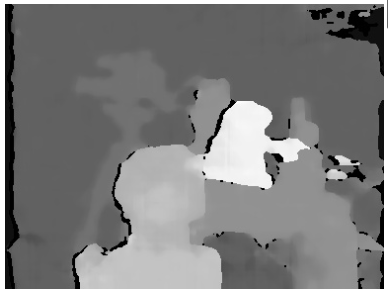
\includegraphics[width=1.2in]{3.png}
}
\subfigure[GC]{
    \includegraphics[width=1.2in]{4.png}
}
\caption{Disparity map}
\end{figure}
\begin{figure}
  \centering
  % Requires \usepackage{graphicx}
  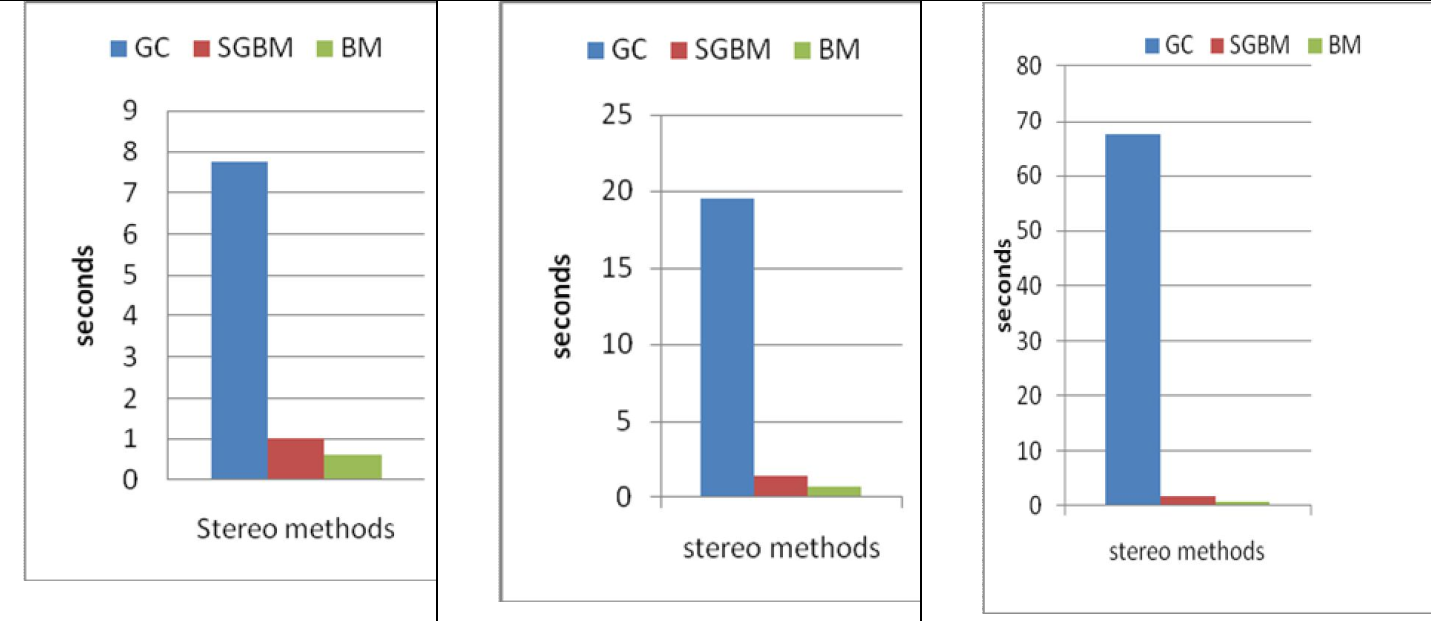
\includegraphics[width=0.8\textwidth]{r2.png}\\
  \caption{Efficiency}
\end{figure}

\indent After obtaining the correspondence between points $p_l$ and $p_r$, calculate the coordinates of $p_l(x_l,y_l)$ in the left camera's coordinate system $x_lOy_l$ and $p_r(x_r,y_r)$ in the right camera's coordinate system $x_rOy_r$. Then the parallax\footnote{always use \textbf{disparity} stands for the estimated parallax} \textbf{$d$ equals to $x_l-x_r$}.

\section{Results}
In this section, we list the methods used in \cite{liu2009distance,patel2013distance,li2016vehicle,sun2019distance} and their experimental results.\\
\indent In \cite{liu2009distance}, Zhengzhen Liu et al. first use smooth filter to the images in order to reduce the noise influence. Then take Canny edge detection and Harris corner detection to find the initial candidate match relations. Then delete impossible match relations according to polar line restraint and gray values' similarities. The result is shown in Table. 1.\\
\begin{table}[!htbp]
\centering
\caption{\textit{Results of \cite{liu2009distance}}}
\begin{tabular}{|c|c|c|}
\hline
The actual distance(m)    & The measured distance(m) & Error \\ \hline
0.7  &  0.661      & 5.57                \\ \hline
1.0  &  0.998       &  1.2            \\ \hline
1.5  &  1.513       &  0.87            \\ \hline
3.0  &  2.996       & 1.13             \\ \hline
5.0  &  5.062       & 1.24             \\ \hline
6.0 &  6.078       & 1.30              \\ \hline
7.5 &  7.784       & 3.79             \\ \hline
\end{tabular}
\end{table}
\indent In \cite{patel2013distance}, Dhaval K. Patel et al. use traditional method to solve the matching problem. They identified the object in two pictures according to its color, and obtained its centroid through geometric calculations. Then directly match the centroids. The disadvantage of this method is apparent: we can only get one pair of matchings and cannot get whole depth information. The result is shown in Table 2.\\
\begin{table}[!htbp]
\centering
\caption{\textit{Results of \cite{patel2013distance}}}
\begin{tabular}{|c|c|c|}
\hline
The actual distance(cm)    & The measured distance(cm) & Error \\ \hline
12  &  12.34      &2.83              \\ \hline
18  &  18.28       &  1.56            \\ \hline
24 &  24.35       &  1.46           \\ \hline
30  &  30.63      & 2.10             \\ \hline
36  &  36.75     & 2.08            \\ \hline
40 &  41.30      & 3.24             \\ \hline
50 &  51.95     & 3.90             \\ \hline
100 &  104.91      & 4.91             \\ \hline
130 & 134.20      & 3.23            \\ \hline
150 &  147.62      & 1.59            \\ \hline
\end{tabular}
\end{table}
\indent In \cite{li2016vehicle}, Yongjie Li et al. use binocular camera to take pictures of a tested vehicle and calculate the vehicle distance. Specifically, they first do camera calibration and then, they take Harris algorithm to extract image corners of the tested vehicle based on gray scale information and then use gray scale distribution to evaluate the similarity of the two images. The matching result is shown as Fig. 5. And Table. 3 shows the experimental results.\\
\begin{figure}
  \centering
  % Requires \usepackage{graphicx}
  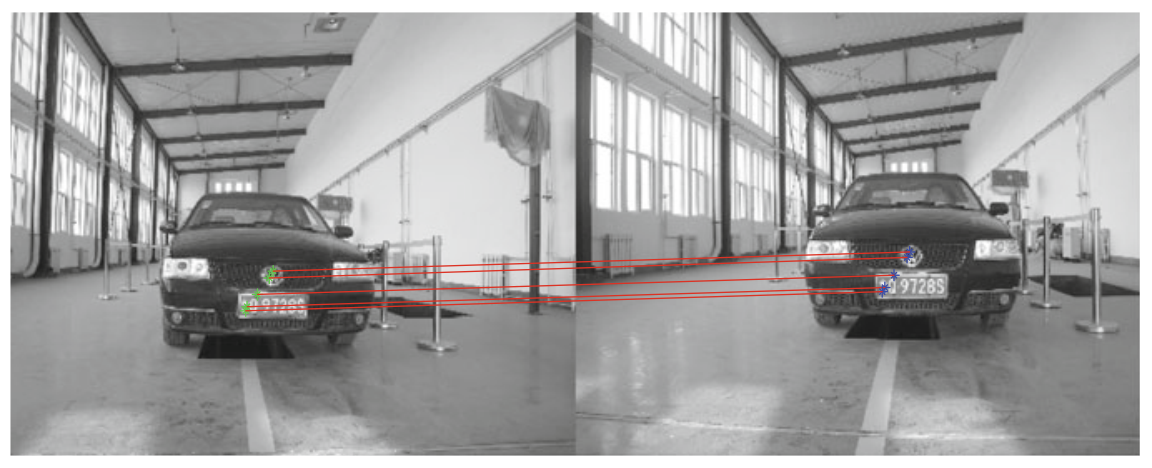
\includegraphics[width=0.8\textwidth]{match.png}\\
  \caption{The matched corners}
\end{figure}
\begin{table}[!htbp]
\centering
\caption{\textit{Results of \cite{li2016vehicle}}}
\begin{tabular}{|c|c|c|}
\hline
The actual distance(m)    & The measured distance(m) & Error \\ \hline
2.4549  &  2.4498      &0.21             \\ \hline
2.4549  &  2.4562       & 0.05            \\ \hline
2.4549 &  2.4675      &  0.51          \\ \hline
2.4549  & 2.4391      &0.64            \\ \hline
2.4549  &  2.4621    & 0.29            \\ \hline
\end{tabular}
\end{table}

\indent As for \cite{sun2019distance}, an area-based matching algorithm of "absolute error accumulation" has been used. The basic idea of this algorithm is to sum the absolute values of the differences between the corresponding values of each pixel, and evaluate the similarity of the two image blocks accordingly. This method is called \textbf{SAD}. Table. 4 shows the experimental results.
\begin{table}[!htbp]
\centering
\caption{\textit{Results of \cite{sun2019distance}}}
\begin{tabular}{|c|c|c|}
\hline
The actual distance(mm)    & The measured distance(mm) & Error \\ \hline
300  &  302.32      &0.77             \\ \hline
300  &  302.23       & 0.74            \\ \hline
500 &  506.74      &  1.33          \\ \hline
500  & 506.89      &1.36            \\ \hline
800  &  815.41    & 1.89            \\ \hline
800  &  815.99      &1.96             \\ \hline
1000  &  1026.27       & 2.56            \\ \hline
1500 &  1555.05      &  3.54          \\ \hline
2000  & 2099.32      &4.73            \\ \hline
2500  &  2665.53    & 6.21            \\ \hline
\end{tabular}
\end{table}
%\indent As for \cite{yang2017analysis}

\subsection{Error Analysis}
Measurement error is mainly from the following two reasons:
\begin{itemize}
\item fabrication error: it is difficult to strictly ensure that the optical axes of two cameras are parallel, the focal length are the same and so on\cite{wenyao2002photoelectric}.
\item image match error: we still need to improve the accuracy and robustness of existing matching algorithm.
\end{itemize}
%\begin{figure}[htbp]
%\centering
%\subfigure[1-bit]{
%    \includegraphics[width=2.5in]{differentBitACC/1.pdf}
%}
%\subfigure[2-bit]{
%    \includegraphics[width=2.5in]{differentBitACC/2.pdf}
%}
%\quad
%\subfigure[3-bit]{
%    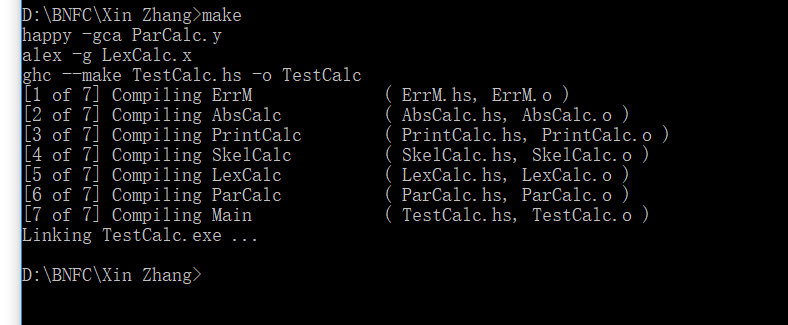
\includegraphics[width=2.5in]{differentBitACC/3.pdf}
%}
%\subfigure[4-bit]{
%    \includegraphics[width=2.5in]{differentBitACC/4.pdf}
%}
%\quad
%\subfigure[8-bit]{
%    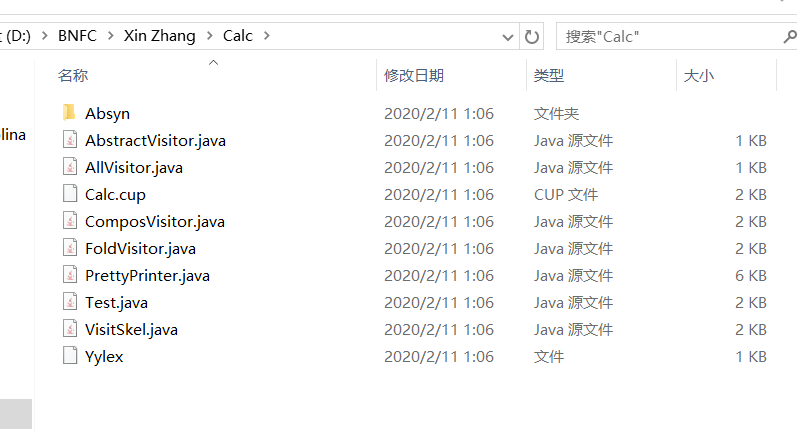
\includegraphics[width=2.5in]{differentBitACC/8.pdf}
%}
%\subfigure[16-bit]{
%    \includegraphics[width=2.5in]{differentBitACC/16.pdf}
%}
%\subfigure[32-bit]{
%    \includegraphics[width=2.5in]{differentBitACC/32.pdf}
%}
%\caption{The accuracy of QNN model trained with different bit numbers}
%\end{figure}

%\begin{table}[!htbp]
%\centering
%\caption{\textit{loss}}
%\begin{tabular}{|c|c|c|c|}
%\hline
%  \diagbox{\textbf{Bit}}{\textbf{loss}}{\textbf{Layer}}    & layer=1 & layer=2 & layer=3 \\ \hline
%1bit  &  0.3600      & 0.3600        & 0.3600         \\ \hline
%2bit  &  0.1888       &  0.1228       & 0.0658        \\ \hline
%3bit  &  0.1468       &  0.0774       & 0.0232       \\ \hline
%4bit  &  0.1310       & 0.0411        & 0.0077        \\ \hline
%8bit  &  0.1221       & 0.0166        & 0.0031        \\ \hline
%16bit &  0.1241       & 0.0160        & 0.0031        \\ \hline
%32bit &  0.1227       & 0.0154        & 0.0031        \\ \hline
%\end{tabular}
%\end{table}
\bibliography{reference}
\end{document}  %�������














